\documentclass[11pt]{article}

\usepackage[margin=0.70in]{geometry}
\usepackage{amsmath,amssymb,graphicx,enumitem,booktabs,array}
\setlist[enumerate]{leftmargin=*,itemsep=7pt,topsep=4pt}

\begin{document}
\begin{center}\textbf{CFD interpretation practical: transonic airfoil screening}\end{center}

\section*{Instructions and reference material}
You have \textbf{30 minutes}. Work individually. No calculator, network access, AI tool, code, or notes are permitted. Show a short calculation where requested; concise evidence-based statements are sufficient elsewhere.

\section*{Scenario}
A $625\ \mathrm{kg}$ high-subsonic cargo UAV, including its payload, is screened at one flight condition. The results below come from a two-dimensional inviscid finite-volume airfoil calculation. Three 12\%-thick candidate configurations have different camber and incidence.

\section*{Reference relations}
Use $g=10\ \mathrm{N/kg}$ and the supplied load factor $n=1.2$:
\[
W=mg,\qquad L_{\rm req}=nW,\qquad L=q_\infty S C_L,\qquad D=q_\infty S C_D.
\]
For this problem, $q_\infty S=10.0\ \mathrm{kN}$. The strong-shock screening limit is
\[
M_{\rm surface,max}\leq1.60.
\]
\noindent A rapid decrease in Mach number paired with a sharp pressure recovery in a surface $C_p$ curve indicates a shock. A strong shock can raise transonic wave drag and may cause separation in a real viscous flow.

\noindent\textbf{Model boundary.} The CFD coefficients are used here as a simplified wing-screening approximation. They do not certify viscous drag, separation, three-dimensional effects, structural loads, stability, or full aircraft performance.

\newpage
\section*{1. Requirements and preliminary recommendations \hfill [10 points]}
\begin{center}
\renewcommand{\arraystretch}{1.35}
\begin{tabular}{c|c|c|c|c|c}
Candidate & Camber & $\alpha$ & $C_L$ & $C_D$ & $M_{\rm surface,max}$ \\
\hline
A: NACA 4412 & high & $2.25^\circ$ & 0.958 & 0.166 & 1.70 \\
B: NACA 2412 & moderate & $1.75^\circ$ & 0.799 & 0.110 & 1.56 \\
C: NACA 1412 & low & $1.50^\circ$ & 0.627 & 0.079 & 1.46 \\
\end{tabular}
\end{center}

\noindent\textbf{Engineer A:} ``Select A. It has the greatest lift coefficient and therefore the greatest payload margin.''

\noindent\textbf{Engineer B:} ``Select C. It has the smallest drag coefficient and therefore is the most efficient choice.''

\begin{enumerate}
\item[1.] (2 points) Calculate $L_{\rm req}$ and $C_{L,\rm req}$.
\item[2.] (2 points) Calculate Candidate B's predicted lift and drag.
\item[3.] (4 points) For each candidate, classify it as \emph{satisfies both requirements}, \emph{fails lift only}, \emph{fails the strong-shock limit only}, or \emph{fails both}. Give one numerical reason for each classification.
\end{enumerate}

\begin{enumerate}
\item[4.] (2 points) In one sentence each, state why Engineer A's and Engineer B's recommendations are incomplete.
\end{enumerate}

\section*{2. Flow-field evidence \hfill [7 points]}
\begin{center}
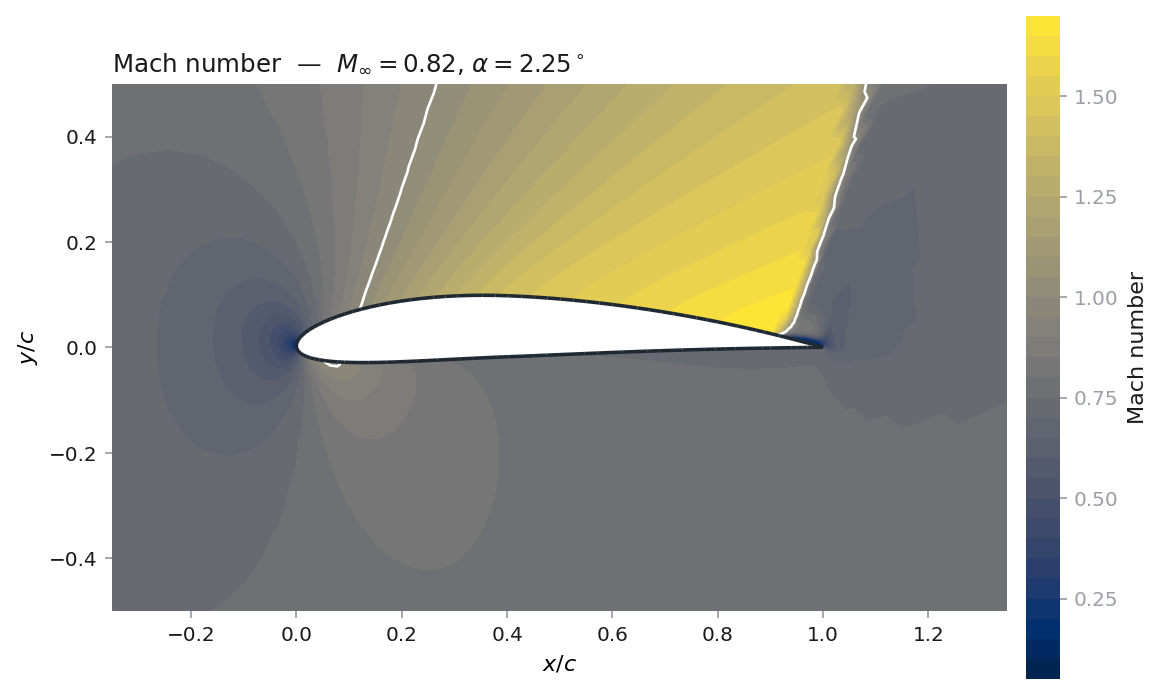
\includegraphics[width=.47\linewidth]{course/week2_figures/candidate_A_mach.png}\hfill
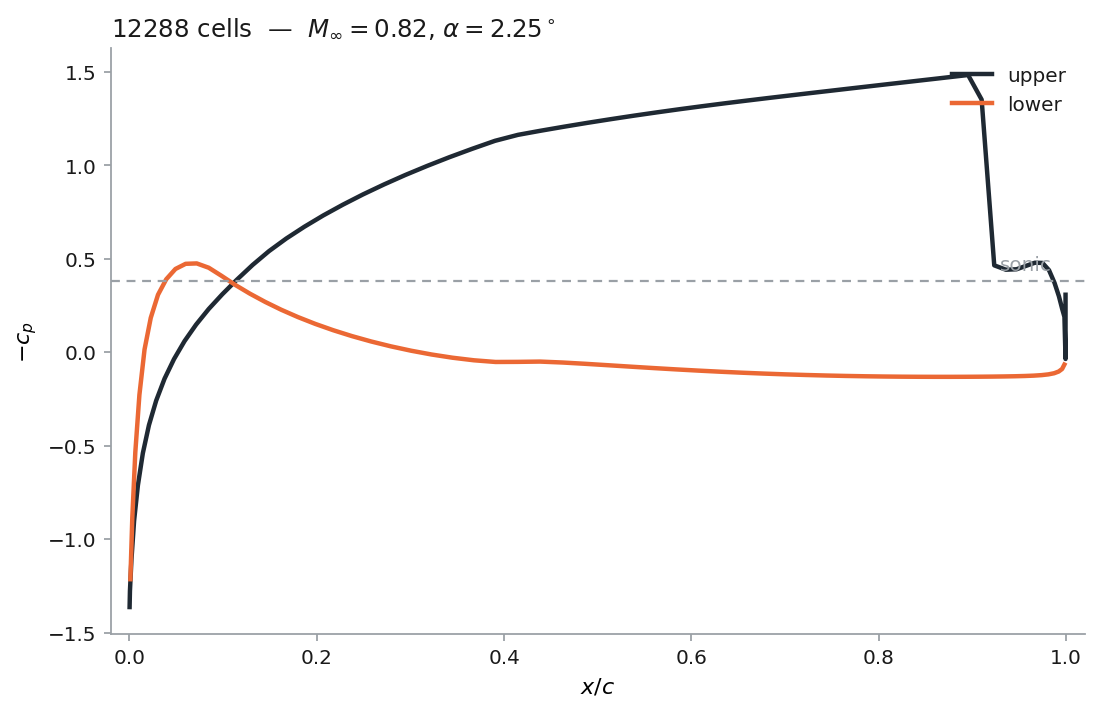
\includegraphics[width=.47\linewidth]{course/week2_figures/candidate_A_cp.png}
\end{center}

\noindent\textit{Candidate A: NACA 4412 at $M_\infty=0.82$ and $\alpha=2.25^\circ$. These are the custom course results used in this practical.}

\begin{enumerate}
\item[5.] (2 points) On the supplied Mach and $C_p$ plots, mark the shock location.
\item[6.] (3 points) Explain how increasing aerodynamic loading can increase lift while also producing a stronger shock and higher drag. Cite one observation from a Mach contour and one observation from a $C_p$ curve.
\item[7.] (2 points) Explain why Candidate A must be rejected despite its large $C_L$.
\end{enumerate}

\newpage
\section*{3. JAX sweep and design recommendation \hfill [9 points]}
\begin{center}
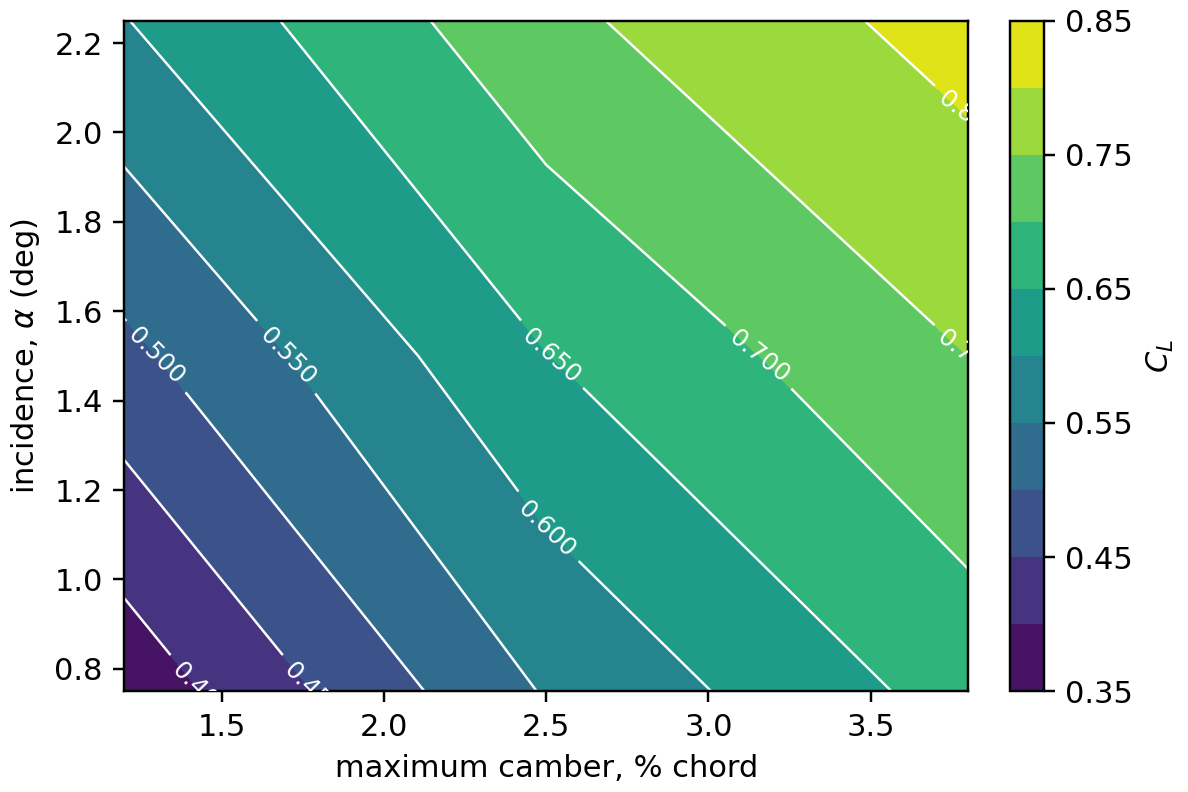
\includegraphics[width=.32\linewidth]{course/week2_figures/jax_cl_map.png}\hfill
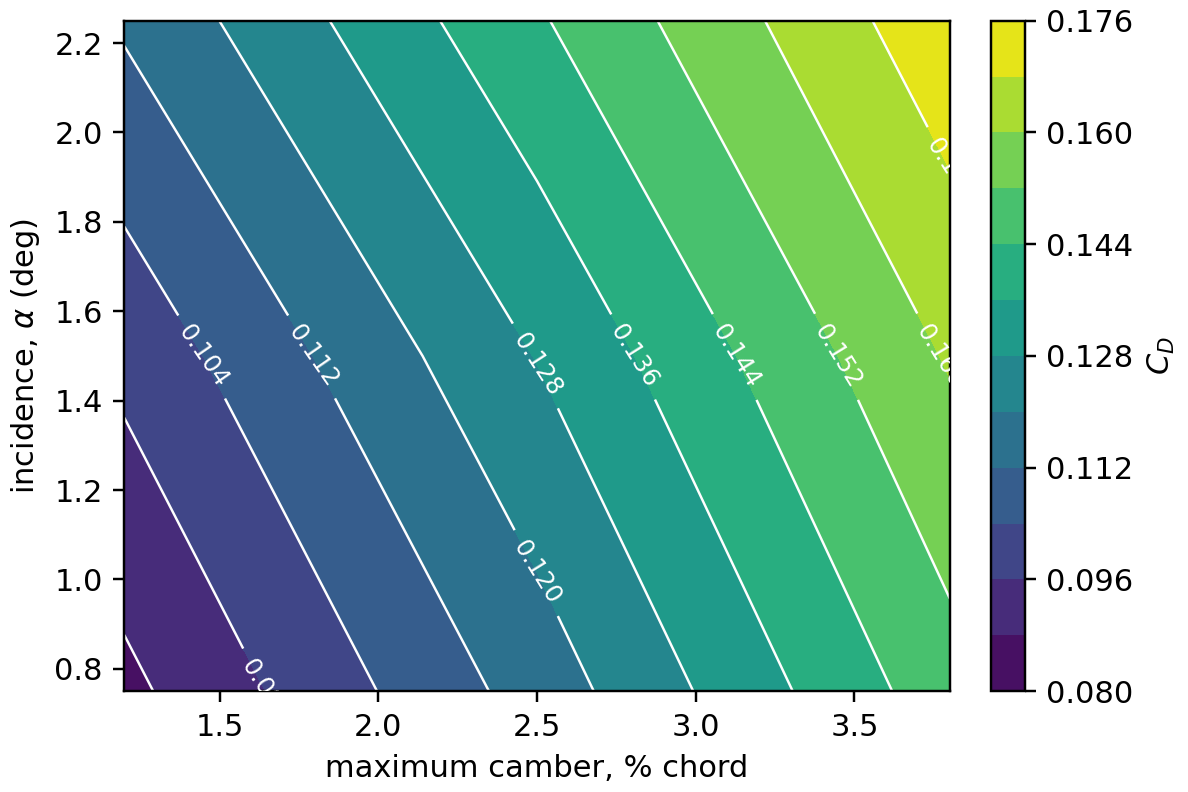
\includegraphics[width=.32\linewidth]{course/week2_figures/jax_cd_map.png}\hfill
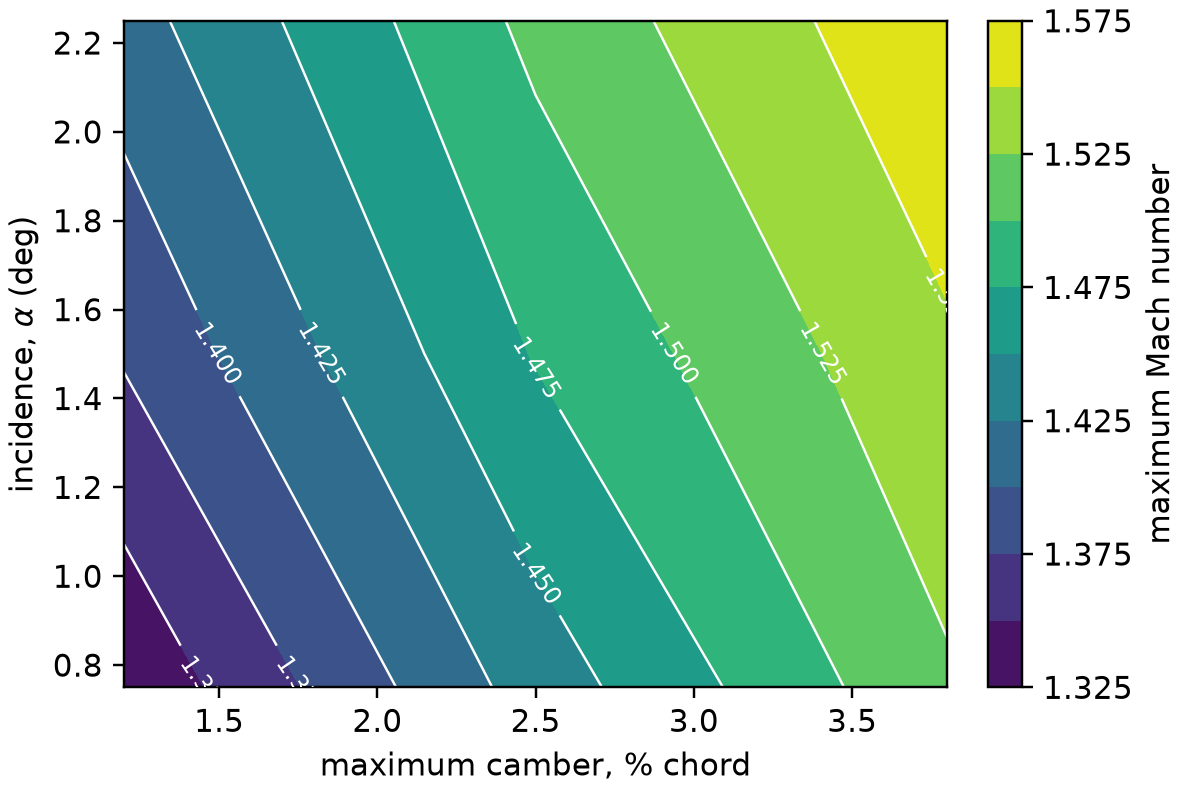
\includegraphics[width=.32\linewidth]{course/week2_figures/jax_mach_map.png}
\end{center}

\noindent\textit{Custom JAX-adjoint screening sweep: fixed 12\% thickness and camber crest at $x/c=0.40$. The black solid line marks $C_L=0.75$; the black dashed line marks $M_{\rm max}=1.60$. Dark-to-light shading uses the colorblind-safe cividis scale.}

\begin{enumerate}
\item[8.] (2 points) Identify the feasible region of the $(m,\alpha)$ sweep: it must meet both the lift and strong-shock requirements. Why is the upper-right portion of the sweep not automatically the best design region?
\item[9.] (2 points) The supplied custom results use one mesh. State the next numerical check required before treating the drag ranking as reliable, and explain why.
\item[10.] (5 points) Use all three maps to choose an approximate $(m,\alpha)$ point that minimizes $C_D$ while meeting $C_L\geq0.75$ and $M_{\rm max}\leq1.60$. State approximate $C_L$, $C_D$, and $M_{\rm max}$ values at that point; explain the trade-off with a nearby equal-lift alternative; and state the next simulation or experiment, with its purpose.
\end{enumerate}

\newpage
\section*{Answer key (instructor review)}
\noindent These are the expected conclusions. Award credit for concise, physically supported equivalents.

\begin{enumerate}
\item[1.] $W=625(10)=6250\ \mathrm{N}$; $L_{\rm req}=1.2(6250)=7500\ \mathrm{N}=7.5\ \mathrm{kN}$; therefore $C_{L,\rm req}=7.5/10.0=0.75$.
\item[2.] For B, $L=10.0(0.799)=7.99\ \mathrm{kN}\approx8.0\ \mathrm{kN}$ and $D=10.0(0.110)=1.10\ \mathrm{kN}$.
\item[3.] A fails the strong-shock limit only: $C_L=0.958>0.75$, but $M_{\rm max}=1.70>1.60$. B satisfies both: $C_L=0.799>0.75$ and $M_{\rm max}=1.56<1.60$. C fails lift only: $C_L=0.627<0.75$, although $M_{\rm max}=1.46<1.60$.
\item[4.] Engineer A ignores the shock constraint and the associated wave-drag risk. Engineer B ignores the required payload lift: C does not meet it.
\item[5.] Mark the abrupt upper-surface Mach decrease near the trailing portion of the airfoil (approximately $x/c=0.9$--$1.0$), paired with the sharp $C_p$ recovery.
\item[6.] Greater camber/incidence increases circulation and upper-surface acceleration, raising lift. The high-Mach region over the upper surface then recompresses abruptly near the shock; the $C_p$ curve shows the corresponding sharp recovery. This creates wave-drag risk (and, in real viscous flow, possible separation).
\item[7.] A produces adequate lift but violates $M_{\rm max}\leq1.60$: its value is 1.70, indicating an unacceptably strong shock by this screen.
\item[8.] The feasible region is the intersection of the $C_L\geq0.75$ side of the solid contour and the $M_{\rm max}\leq1.60$ side of the dashed contour. The upper right is not automatically best because increasing camber and incidence raises drag and eventually violates the shock constraint.
\item[9.] Perform a grid-refinement (mesh-convergence) study, comparing $C_L$, $C_D$, and shock location/strength over progressively finer meshes. Drag and shocks can be sensitive to numerical resolution, so one mesh cannot establish a reliable ranking.
\item[10.] Accept a point on the minimum-$C_D$ portion of the feasible boundary, supported by approximate readings from all three maps. It should meet both constraints; a higher-camber/lower-incidence equal-lift alternative generally has different drag and shock margin. The next step should be, for example, a mesh-refined viscous CFD calculation (or a wind-tunnel test) to assess drag, shock/boundary-layer interaction, and separation before a design decision. \textit{After regenerating the maps, replace this sentence with the selected numerical reference point and tolerances for grading.}
\end{enumerate}
\end{document}

